\documentclass[runningheads]{llncs}

\linespread{1.1}

\raggedbottom

\usepackage{float}

\usepackage{lmodern}
\usepackage[english]{babel}

\usepackage{fontspec}
\defaultfontfeatures{Ligatures=TeX}

\usepackage{multicol}

\usepackage{listings}

\usepackage{datetime}
\setdefaultdate{\usdate}

\usepackage{graphicx}
\graphicspath{{assets/}}

\newcommand{\german}[1]{{#1}}

\title{Low-Code vs.\texorpdfstring{\\}{} Model-Driven Architecture}
\author{Markus Reiter}


\PassOptionsToPackage{hyphens}{url}
\usepackage{hyperref}
\usepackage[nameinlink, noabbrev]{cleveref}
\usepackage{nameref}

\addto\extrasenglish{
  \def\sectionautorefname{Section}
}

\usepackage[
  style   = numeric,
  sorting = none,
]{biblatex}
\bibliography{paper}

\begin{document}

\institute{University of Innsbruck, Austria}

\maketitle

\vspace{8em}

\begin{abstract}

In this paper we present a survey conducted by comparing low-code tools with model-driven tools for developing software in order to get a better understanding of the advantages and drawbacks of both approaches and whether they are a viable alternative to traditional software development.

\keywords{Low-Code \and Model-Driven \and Development}

\end{abstract}

\newpage

\section{Introduction}
\label{sec:introduction}

In this paper, we compare Low-Code Platforms to Model-Driven Architecture and try to determine when and where to use them over Model-Driven Architecture or vice-versa.

In order to make clear to the reader the difference between the two approaches we firstly provide definitions and characteristics of each paradigm in the following sections.

\subsection{What is Model-Driven Architecture?}
\label{ssec:what_is_model_driven}

With Model-Driven Architecture or Model-Driven Engineering, the goal is to standardise on models in a given domain. This is done in order to reduce code duplication and speed up development. Especially when bootstrapping a new project, it is helpful keep boilerplate code to a minimum. In addition to reducing development time, Model-Driven Engineering also tries to increase productivity by maximising compatibility between systems by using the aforementioned standardised models.~\cite{wiki:model_driven_engineering} Generally, Model-Driven Architectures are geared towards developers, i.e. people who also have a good understanding of the underlying programming language(s) of the respective architecture. One common way Model-Driven Engineering is used in practice is code generation. Using code generation can speed up many processes: For example, given an API specification (e.g. using the industry standard OpenAPI~\cite{openapis}), one can generate all code that is necessary for a client for this API. Swagger~\cite{swagger} is one such tool which can generate API clients for many different programming languages. There are also tools which can generate a complete class hierarchy from an UML diagram; many IDEs offer such functionality either natively or via plug-ins. These are only a few examples of what falls into the category of Model-Driven Architecture, the main point is that all of them help developers reach their goal faster than doing the same tasks manually.

\subsection{What is a Low-Code Platform?}
\label{ssec:what_is_a_low_code_platform}

A low-code platform, as the name implies, requires a minimal amount of code to be written. Similarly to conventional programming (i.e. using a programming language), an IDE is used for creating programs using low-code platforms. Often, the IDE is part of the low-code platform itself instead of a standalone program as is the case for conventional programming. In most cases, the IDE of the platform and the low-code platform cannot be used separately so the term low-code platform is also commonly used to refer to the IDE interface itself. Low-code platforms are targeted towards users with little to no programming experience, which means the actual programming of a low-code system is done mainly via visual building blocks. These building blocks contain pre-built templates and functionality and can be combined to form a coherent user interface. Oftentimes, custom functionality can be implemented using a click-and-drag pattern between building blocks and by assigning an action accordingly. The available building blocks vary by platform which makes them less portable than a system written using a programming language. This is one common point of critique on low-code platforms.

Another sub-category of low-code platforms are so called no-code platforms~\cite{wiki:no_code_development_platform}. Where to draw the line between low-code and no-code is not clearly defined, especially since low-code platforms can sometimes be used in a way that cannot be differentiated from no-code platforms. For the purposes of this paper, low-code platforms are general purpose visual programming languages~\cite{wiki:visual_programming_language} aimed at both developer and non-developer users while no-code platforms are closer to software as a service (SaaS) platforms targeted mostly (or only) towards non-developers. Another way to look at it is that low-code platforms still give developers the freedom to add custom building blocks for their specific use case and no-code solutions are usually purpose-made for a specific line of business or a specific type of department. Some examples include monday.com~\cite{wiki:monday_com}, a no-code platform for project management tasks; FileMaker~\cite{wiki:filemaker}, which provides a database engine and a corresponding no-code platform for creating graphical user interfaces for interacting with databases; and Airtable~\cite{wiki:airtable}, a no-code platform for creating databases connected to interactive spreadsheets.

\section{Evaluation of Low-Code Tools}
\label{sec:evaluation_of_low_code_tools}

\subsection{Selection of Low-Code Tools}
\label{subsec:choosing_low_code_tools}

Before evaluating low-code tools, we had to first determine which tools to evaluate. Given the ever evolving landscape of low-code platforms, there are countless companies offering low-code solutions. The following is an incomplete list of low-code platforms we found:

\begin{itemize}
  \item Oracle APEX (Application Express) (originally released as Oracle Flows in 2000) by Oracle (founded in 1977)
  \item OutSystems (founded in 2001)
  \item Mendix (founded in 2005), a subsidiary of Siemens
  \item Simplifier (founded in 2012 as iTiZZiMO, renamed 2019 to Simplifier, the same name as its low-code platform)
  \item OSBP (Open Standard Business Platform), an open-source low-code platform (developed since 2016) under the umbrella of the Eclipse Foundation
  \item Corteza Low Code, part of the open-source Corteza Project (released in 2019), originally developed by Crust Technology
\end{itemize}

We wanted our evaluation to contain at least one open-source platform (e.g. OSBP), one platform backed by a well-known corporation (e.g. Oracle), one platform by a relatively new/unknown corporation (e.g. Simplifier), one relatively old/well-established platform (e.g. Oracle APEX or OutSystems) and one relatively new platform (e.g. Simplifier or Corteza). With the given list of low-code platforms, we could satisfy this requirement.

To ensure we could properly test all of these tools, we conducted a brief first inspection of each. Therefore, the following section will give a brief explanation of each platform, any problems encountered during the initial setup and the steps necessary before being able to use the low-code platform.

\subsubsection{OSBP (Open Standard Business Platform)}

The Open Standard Business Platform is an open-source development environment which combines no-code and low-code with traditional application development.~\cite{osbp} It is the community version of OS.bee~\cite{osbee}, a commercial product developed by COMPEX only available to business users. The interface for the OSBP platform is implemented via a plug-in for the Eclipse IDE. The user first needs to install the Eclipse IDE, after which they can add the link to the plug-in repository and install it directly from within the IDE. Unfortunately, the latest version of OSBP was released more than one year ago and is incompatible with the latest version of the Eclipse IDE. At the time of writing (Jan 2, 2021), the last commit in the OSBP Git repository was on May 9, 2019. The latest version of the Eclipse IDE was 2020-12. The OSBP website recommended downloading Eclipse Neon, a version of the Eclipse IDE released in 2016. A non-functioning IDE plug-in for an outdated version of said IDE which has not been updated in over a year is a red flag. We therefore deemed OSBP unsuitable and decided to exclude it from further evaluation.

\subsubsection{Corteza}

Corteza Low Code is part of the Corteza Project~\cite{corteza} initiated by Crust Technology. The Corteza Project encompasses Corteza CRM Suite, an open-source customer relationship management tool built entirely on Corteza Low Code; Corteza Messaging, a messaging solution similar to the likes of Slack; Corteza One, a unified workspace from which to access and run web applications and finally Corteza Low Code, a low-code platform designed for building record-based applications. It is possible to try out Corteza directly in the browser by creating an account or by using an existing GitHub or Google account to sign up. We chose to set up a local demo deployment using Docker. The Corteza Project provides very good documentation on how to get started, including a ready-made \texttt{docker-compose.yml} file containing all necessary services for a full Corteza installation. After a simple call to \texttt{docker-compose up -d}, the Corteza server was running locally. The last step before being ready to use was to set up an administrator account in the local Corteza instance.

\subsubsection{Oracle APEX (Application Express)}

Oracle Application Express~\cite{oracle_apex} is a web-based application development platform developed by Oracle. It is backed by an Oracle database and allows building web applications using a low-code interface. Oracle offers three ways to set up APEX. The first is to use it as part of their Oracle Cloud offering, secondly, by requesting a free workspace or lastly by self-hosting using the Oracle APEX On Premise variant. For our purposes, we chose to request a free workspace for testing. We chose a name for our namespace and registered using an email address and shortly thereafter we were sent an approval email with the login details. After that, Oracle APEX was ready to use.

\subsubsection{Simplifier}

Simplifier is, like Oracle APEX, a web-based application development environment on low-code basis. Simplifier offers a demo platform called “Simplifier Playground”, an instance of the Simplifier platform specifically set up for trialling the platform. The trial instance is reset to defaults every night, so all data stored on it will not be persisted. They also offer a “Freemium” instance, available by registering via an email address, which has no such limitation, we therefore applied for such an instance. %TODO

\subsubsection{Mendix}

Similar to Oracle APEX and Simplifier, Mendix is also a web-based environment for low-code application development. Mendix offers a free tier which allows hosting unlimited applications with 1GB of memory and 0.5GB of storage per application. For more advanced needs, Mendix offers an enterprise option starting at 1875€ per month, allowing on-premises hosting and hosting on private clouds, e.g. AWS, IBM etc. For our evaluation purposes, the free tier is more than enough given there are no restrictions on the provided functionality. Creating an account was straight-forward and we were able to log in within minutes of registering. There are two options for developing applications using Mendix: The first is the web-based environment called Mendix Studio, the second a native desktop application called Mendix Studio Pro, offering more advanced options for professional users. Unfortunately Mendix Studio Pro is only available for Microsoft Windows, so we were not able to test it, the basic functionality for creating low-code application is the same in both versions of Mendix Studio, however.

\subsection{Developing a TODO List Application}

In order to evaluate each platform, we decided to build a simple TODO list application. The user should be able to add items to the list containing a title, body text and the status of the TODO item (either “done” or “outstanding”).

\subsubsection{Corteza}

\begin{figure}
  \centering
  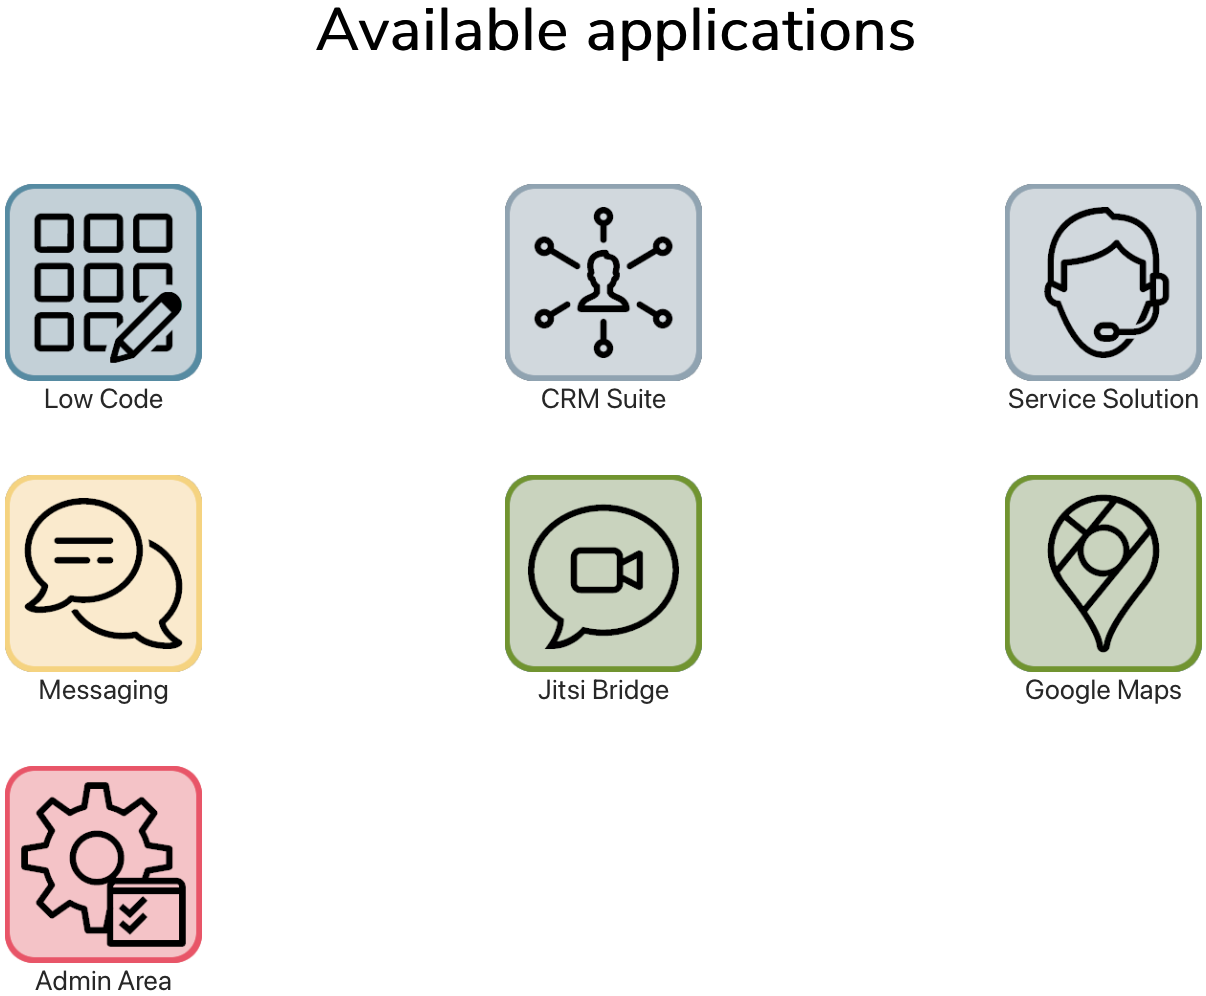
\includegraphics[width=0.6\textwidth]{corteza-home-screen}
  \caption{Corteza Home Screen}
  \label{fig:corteza_home_screen}
\end{figure}

In \cref{fig:corteza_home_screen}, we can see the initial screen of the Corteza platform. By selecting “Low Code”, we reach a new view containing all existing “Low Code Namespaces”. A namespace can be thought of as an individual application within the low-code environment. In order to start with our application, we create a \texttt{todo-list} namespace. Next we need to create a module. A module in Corteza is similar to creating a database schema for a single table. For our application, we create a module containing text fields for \texttt{title} and \texttt{body} and a drop-down field for the \texttt{status}. We also mark \texttt{title} as a required field, as seen in \cref{fig:corteza_module}. Next, we need to create a page which lets us add TODOs to our list. To do this, we create a blank page and add the pre-built “Record List” block. In the “Record List” block, we select our “TODO Module” as the data source and select all fields so they are displayed in the list. The list also provides an option to allow inline editing of records. Without this option, the user has to click on the list item to open the detail page in order to edit it. Unfortunately, for some reason when enabling the checkbox to allow inline editing, we were unable to save the page with this configuration. Nevertheless, the basic functionality of our application was completely implemented in less than ten minutes.

\begin{figure}
  \centering
  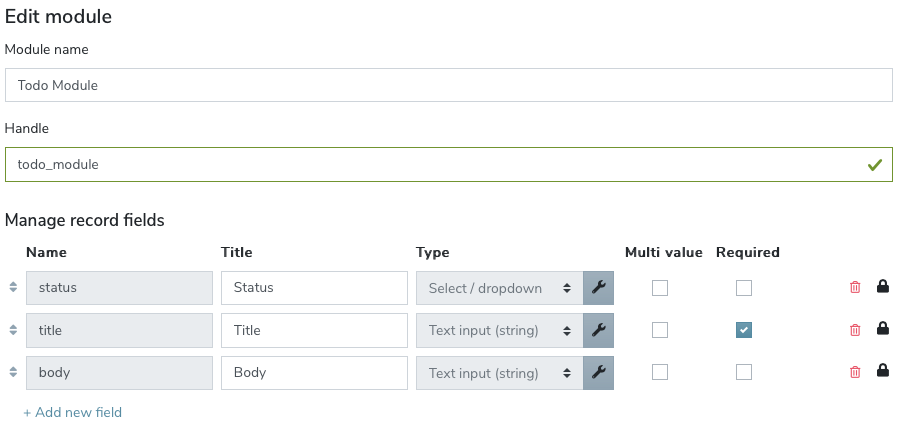
\includegraphics[width=\textwidth]{corteza-module}
  \caption{Creation of a Corteza Module}
  \label{fig:corteza_module}
\end{figure}

There are also some other features in Corteza: The “Chart Builder” allows creating charts for data in a module and it is possible add custom buttons with automations. The custom automations however, have to be fully implemented in JavaScript, so we didn't evaluate them any further given our focus on low-code.

\subsubsection{Oracle APEX (Application Express)}

\begin{figure}
  \centering
  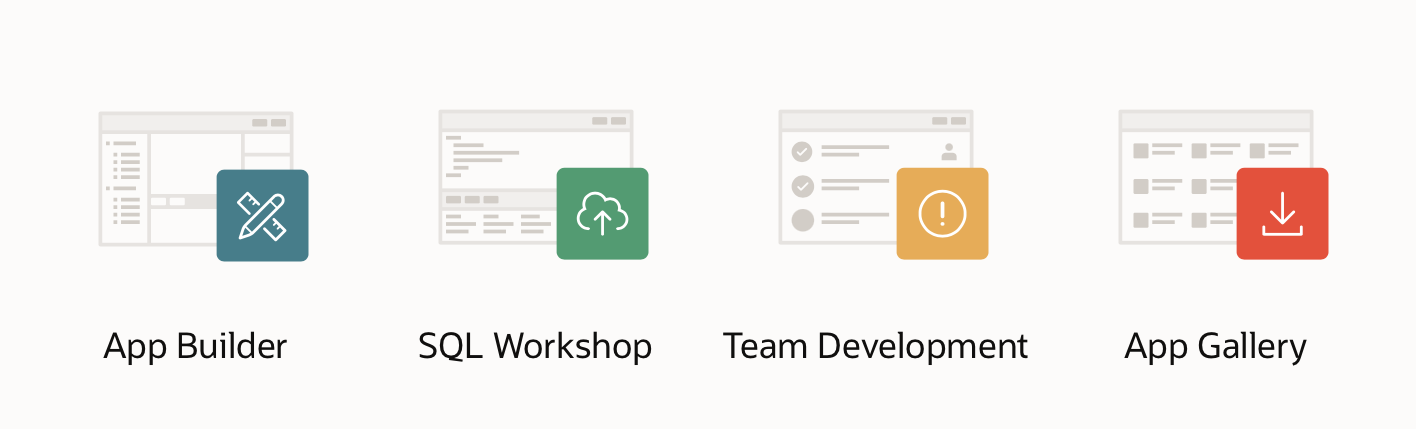
\includegraphics[width=\textwidth]{oracle-apex-home-screen}
  \caption{Oracle APEX Home Screen}
  \label{fig:oracle_apex_home_screen}
\end{figure}

When first logging into Oracle APEX, the user is greeted with a an overview of all applications in the workspace and a quick menu for accessing the major parts, App Builder, SQL Workshop, Team Development and App Gallery, as seen in \cref{fig:oracle_apex_home_screen}. App Builder is the low-code development interface, allowing the user to create page-based web applications, SQL Workshop is an interface to create database tables for use in low-code applications. Team Development is an integrated project management tool that helps coordinate tasks across team members when multiple people are working together in the same namespace. And finally, App Gallery is a gallery containing sample applications to use as either templates or guidance when developing a new low-code application.

Before starting with our TODO list application, we decided to set up a sample application called “Sample Database Application”, which contains a basic inventory management application, including a product list which we used as a template for our TODO list.

For our TODO list, we created a new application called “TODO List”. The setup wizard allows customising the colour theme of the application, the menu style (e.g. side menu or top menu), language as well as the application icon. Once created, we had a blank application containing a login page and a home page. The next thing we needed to do was set up a database table for our TODO items. Basic SQL knowledge is required to do this since properly setting up a primary key and a unique constraint for it is necessary to be able to insert data later on. We now had a \texttt{TODOS} table containing \texttt{ID}, \texttt{STATUS}, \texttt{TITLE} and \texttt{BODY} and were now able to add a new page to our application.

\begin{figure}
  \centering
  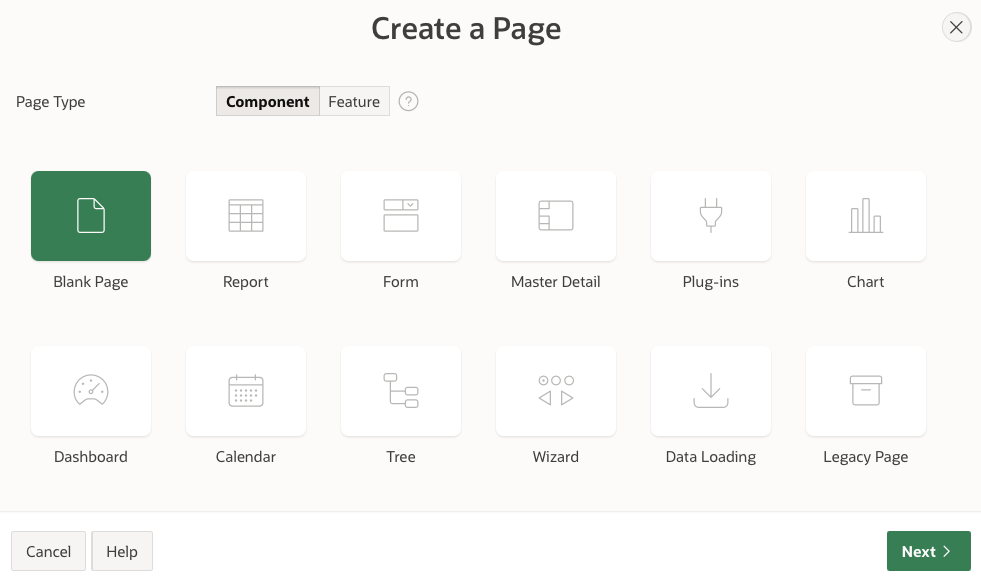
\includegraphics[width=\textwidth]{oracle-apex-create-page}
  \caption{Oracle APEX Create Page Dialog}
  \label{fig:oracle_apex_create_page}
\end{figure}

There are many different page styles to choose from, as seen in \cref{fig:oracle_apex_create_page}. For our use case, we chose the “Form” page template. The user simply assigns a page name and subsequently selects the  corresponding database table. The result is a form page with all fields of the database table which lets the user add new tasks and edit existing ones. Some minor visual adjustments were necessary for the form page, i.e. hiding the automatically generated \texttt{ID} and setting the \texttt{STATUS} to “outstanding” by default when adding a new task. The next step was to create a list containing our TODO items with a button that opens the form page to add new ones. Similar to the page templates, there are many different building blocks to choose from. We used the same as the one used in the sample application, the “Interactive Report”, a table view with filtering options. Lastly, we added a \texttt{CREATE} button to the top of this component, linking it to the form page created earlier.

Oracle APEX provides many advanced options for all building blocks which allows building custom logic by connecting them via events (e.g. mouse click or value change). It is also possible to create custom events: For example, a form page (in dialog form) provides a \texttt{Cancel Dialog} event which is fired when the \texttt{CANCEL} button is pressed.

\subsubsection{Mendix}

Mendix offerse three ways for creating a new application: Creating a blank application from scratch, generating an application from spreadsheet data or using one of many templates as a starting point. For our TODO list application, we chose to create an application from scratch. After creating an application, you can either edit it using the web interface or open it in the Mendix Studio Pro desktop application. We developed our TODO list application entirely using the web interface. The Mendix interface provides four main menu items: Pages, Domain Models, Microflows and Navigation. Pages is used to manage the different pages needed for the application. Domain Models contains the entities for our application, in our case we needed an entity for items in our TODO list. Microflows are used to add custom logic (micro workflows) to the application, e.g. when clicking a button. An interesting feature is Mendix Assist, an AI-based assistant making suggestions to the user when creating Microflows. Lastly we have Navigation, which is simply the representation of the application menu hierarchy.

\begin{figure}
  \centering
  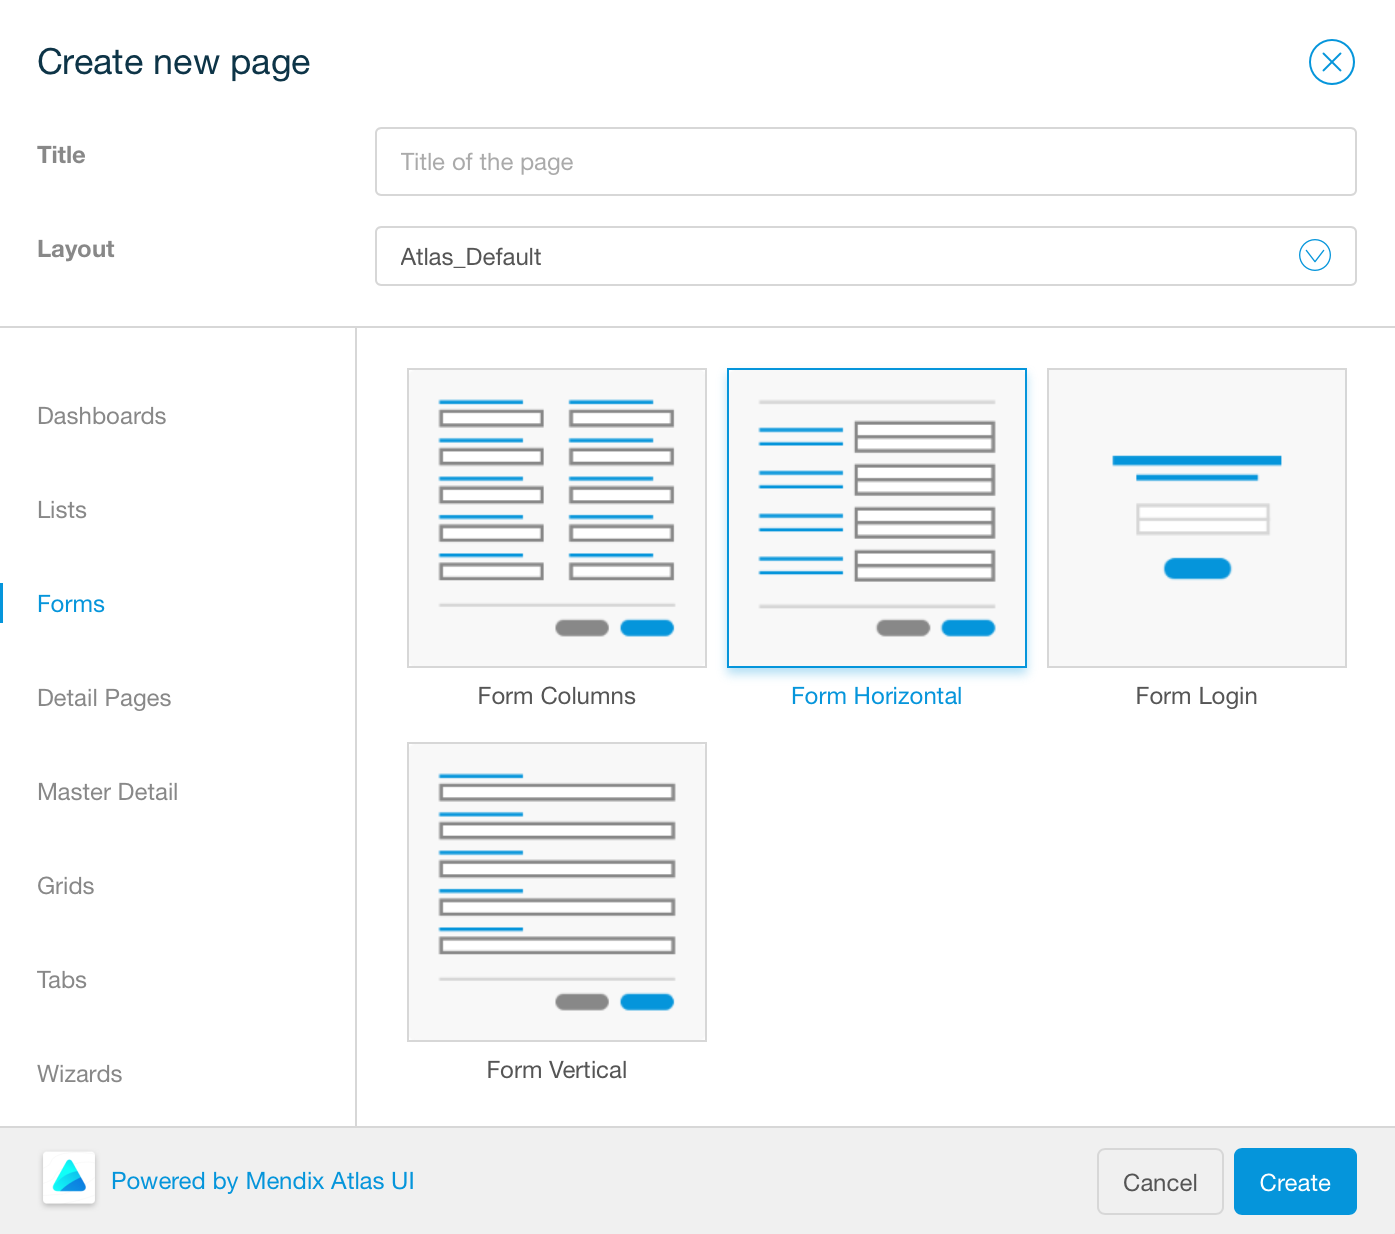
\includegraphics[width=0.8\textwidth]{mendix-create-page}
  \caption{Mendix Create Page Dialog}
  \label{fig:mendix_create_page}
\end{figure}

For our application, we started by adding a new page for creating a task on our TODO list. There are numerous page templates to choose from, we used the “Form Horizontal” template as seen in \cref{fig:mendix_create_page}. The resulting page (\texttt{add\_task}) contains a so called data view. Every data view needs a data source, so we were prompted to create a new entity. We added a new entity called \texttt{task} and while editing the form, we were prompted to add attributes to that entity. We added two \texttt{String} attributes for \texttt{title} and \texttt{body}. We also needed to add a \texttt{status} attribute; for this, we edited the entity directly, adding an attribute of type \texttt{Enumeration} with values for “done” and “outstanding” and set the default value to “outstanding” accordingly.

Next, we added a list view to the \texttt{home} page, choosing the \texttt{task} entity as data source in the process. We could now drag text fields into the list view and choose the corresponding attributes to be displayed. In order to actually add new tasks, we also added a “New task” button. For the click action, the user can choose to open a page or run a microflow or a predefined action such as saving changes on the current page. We chose our page for creating a new task as the target and also needed to enable the “Create object” option. With this option, we pass an empty \texttt{task} object to the page, since the data view on the page expects a \texttt{task} as data source.

Lastly, we created another form page (\texttt{edit\_task}), also containing the \texttt{status}, in order to be able to edit a \texttt{task}. To access it, we added a click event to the list view on the \texttt{home} page. Since the list view data source is a \texttt{task}, it is automatically passed to the data view on the \texttt{edit\_task} page.

\section{Evaluation of Model-Driven Tools}
\label{sec:evaluation_of_model_driven_tools}

\section{Findings}
\label{sec:findings}

\section{Conclusion}
\label{sec:conclusion}

\newpage
\printbibliography

\end{document}
